%-------------------------------------------------------------------------------
%	PAQUETES Y OTRAS CONFIGURACIONES
%-------------------------------------------------------------------------------

%-------------------------------------------------------------------------------
%	PAQUETES Y OTRAS CONFIGURACIONES
%-------------------------------------------------------------------------------
\documentclass{tufte-handout}
%\documentclass[paper=letter, fontsize=11pt]{scrartcl} % Tamaño de papel y letra para el documento
\usepackage{geometry}
\geometry{left=1.2cm, right=6.2cm, top=2.5cm, bottom=2.5cm}
\usepackage{color}
\usepackage[utf8]{inputenc} % Los caracteres acentuados se pueden escribir normalmente en el código
\usepackage[T1]{fontenc} % Configuración de fuente de salida
\usepackage{cmbright}
\usepackage[sfdefault]{noto}
\usepackage[T1]{fontenc}
\normalfont
\usepackage{graphicx} % Paquetes para incluir imágenes
\usepackage{multicol}
\usepackage{circuitikz}
\usepackage{tikz}
\usetikzlibrary{arrows}

\usepackage{sectsty} % Paquete para configuración de secciones
\allsectionsfont{\centering \normalfont \scshape} % Los títulos de las secciones son centrados, con la misma fuente y pequeñas mayúsculas

\usepackage{todonotes}
\usepackage{microtype}
\renewcommand{\figurename}{Figura}

\usepackage{listings}
\renewcommand{\lstlistingname}{Código}
\lstdefinestyle{mystyle}{
    basicstyle=\footnotesize,
    breakatwhitespace=false,
    breaklines=true,
    captionpos=b,
    keepspaces=true,
    numbers=left,
    numbersep=5pt,
    showspaces=false,
    showstringspaces=false,
    showtabs=false,
    tabsize=2
}
\lstset{style=mystyle}

% \usepackage{fancyhdr} % Paquete para personalizar pies y cabeceras de página
% \pagestyle{fancyplain} % Todas las páginas con las mismas cabeceras y pies de página
% \fancyhead{} % Sin cabecera
% \fancyfoot[L]{} % Vacío en la izquierda del pie de página
% \fancyfoot[C]{} % Vacío en el centro del pie de página
% \fancyfoot[R]{\thepage} % Número de página en el pie de pagina
% \renewcommand{\headrulewidth}{0pt} % Sin lineas en la cabecera
% \renewcommand{\footrulewidth}{0pt} % Sin lineas en el pie de página
% \setlength{\headheight}{13.6pt} % Altura de cabecera
%
% \numberwithin{equation}{section} % Numera ecuaciones en cada sección
% \numberwithin{figure}{section} % Numera figuras en cada sección
% \numberwithin{table}{section} % Numera tablas en cada sección
%
% \setlength\parindent{0pt} % Quita la indentación de los párrafos

\newcommand{\horrule}[1]{\rule{\linewidth}{#1}} % Comando personalizado para hacer linea horizontal


%-------------------------------------------------------------------------------
%	TITULO
%-------------------------------------------------------------------------------

\title{Práctica 1 - Equipo de laboratorio\\Interfaces y periféricos para robots}
\author{Roberto Cadena Vega} % Nombre del profesor
\date{}

%-------------------------------------------------------------------------------
%	EMPIEZA EL DOCUMENTO
%-------------------------------------------------------------------------------

\begin{document}
\maketitle % Imprime el título

%-------------------------------------------------------------------------------
%	OBJETIVOS
%-------------------------------------------------------------------------------

\section{Objetivos}

	Familiarizarse con el equipo del laboratorio de electrónica y comprender el funcionamiento del lenguaje de programación Wiring-Arduino.

%-------------------------------------------------------------------------------
%	CONOCIMIENTOS PREVIOS
%-------------------------------------------------------------------------------

\section{Conocimientos Previos}

%-------------------------------------------------------------------------------

	\subsection{Lenguajes de programación para microcontroladores}

		Dentro del encuadre de esta materia se maneja como objetivo de conocimiento el utilizar lenguajes de programación para microcontroladores de alto nivel y de bajo nivel, por lo que resulta bastante conveniente utilizar un ambiente de desarrollo como el de Wiring-Arduino, el cual nos permite empezar a trabajar con un lenguaje de programación de alto nivel, facil de comprender y de dominar, aprendiendo los conceptos importantes del funcionamiento de un $\mu C$ (microcontrolador) y dejar para prácticas posteriores el uso de lenguajes de programación de bajo nivel, con la ventaja de poder utilizar el mismo $\mu C$ con las mismas herramientas de software.

		Por el momento empecemos a revisar el ambiente de desarrollo de Arduino en la figura \ref{fig:arduino-ide}

		\begin{marginfigure}
    	\begin{center}
    		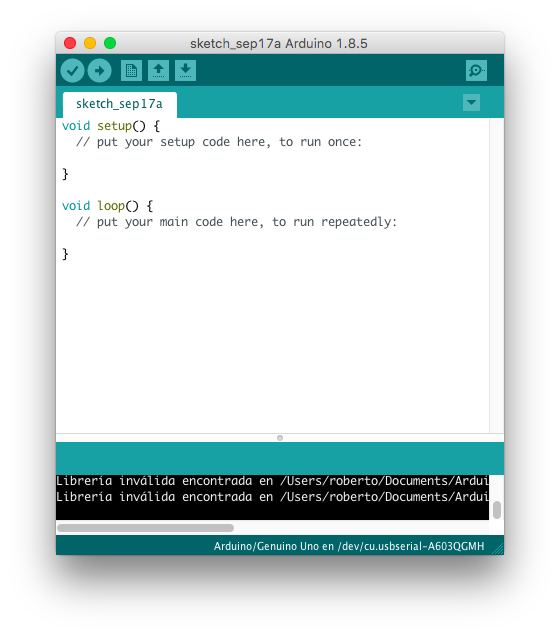
\includegraphics[width=\textwidth]{images/Arduino-IDE.png}
    		\caption{IDE de Arduino}
    		\label{fig:arduino-ide}
    	\end{center}
    \end{marginfigure}

		En la parte superior de la ventana se puede encontrar los siguientes botones:

		\begin{description}
			\item[Verificar] - Este boton manda la orden de compilar el programa para asegurar que no haya errores de compilación.
			\item[Subir] - Este boton manda la orden de compular el programa y envar el archivo binario para la escritura dentro de la memoria del $\mu C$.
			\item[Nuevo] - Abre una nueva ventana del IDE con un archivo nuevo.
			\item[Abrir] - Abre el navegador de archivos para escoger el archivo a abrir.
			\item[Salvar] - Guarda el archivo de la ventana actual.
		\end{description}

		En la parte central de la ventana se encuentra el espacio para redactar el programa a ejecutar y la ventana de mensajes en donde se despliega el estado del compilador.

		En el borde inferior derecho de la ventana se encuentra especificado el modelo de tarjeta de desarrollo a utilizar por el compilador y el puerto especifico en el que esta conectado. Esta información se puede modificar en el menu principal del IDE, en la opción de Herramientas.

		Cuando se abre el IDE de Arduino por primera vez, se tiene el siguiente programa por default:

		\lstinputlisting[language=C]{codigos/inicio.ino}

		En donde podemos ver dos bloques principales para nuestra programación:

		\begin{description}
			\item[setup] - En este función existen las indicaciones para inicializar el $\mu C$, es decir las instrucciones que se ejecutarán en el $\mu C$ solo una vez (cuando el $\mu C$ inicia su operación).
			\item[loop] - En este función existen las instrucciones que se ejecutarán una y otra vez mientras el $\mu C$ este funcionando.
		\end{description}

		Podemos ver un ejemplo de programación en Arduino directamente en los ejemplos del software (en el menu principal, Archivo, Ejemplos, 01.Basics, Blink):

		\lstinputlisting[language=C]{codigos/Blink.ino}

		En las lineas 1 - 23 se tiene un comentario de multiples lineas, en la linea 25 se tiene un comentario de una sola linea.

		En la linea 28, adentro de la función setup, se tiene la inicialización de un pin del puerto de salida de la tarjeta de desarrollo, en donde se configura el pin LED\_BUILTIN, como un pin de salida, es decir, se configura de tal manera que el pin pueda cambiar el voltaje de acuerdo a la programación a continuación\footnote{Lo contrario sería configurar el pin como entrada, lo cual dejaría al programa sin la capacidad de modificar el voltaje en este, pero con la capacidad de leer un voltaje causado por una fuente externa.}.

		En la linea 33, adentro de la funcion loop, se cambia el estado del pin LED\_BUILTIN a alto, lo que hará que el pin físico del $\mu C$ asociado a LED\_BUILTIN\footnote{En las lineas iniciales de comentarios se describe a LED\_BUILTIN como el pin 13 para las tarjetas de desarrollo más comúnes de Arduino, por lo que si se reemplaza LED\_BUILTIN con 13, el funcionamiento de este programa será el mismo.} tenga un voltaje de $5V$, en la linea 34 se llama a la función delay con un argumento de $1000$, la cual hará que el $\mu C$ espere $1000 ms$ o bien $1s$, en la linea 35 se cambia el estado del pin LED\_BUILTIN a bajo, con lo que el pin físico del $\mu C$ asociado a LED\_BUILTIN tenga un voltaje de $0V$ y en la linea 36 se llama a la función delay para esperar $1s$.

		El resultado final de este programa será que el $\mu C$ encenderá y apagará el LED instalado en la misma placa de desarrollo con intervalos de $1s$.

		En el siguiente ejemplo se describe como leer el voltaje del pin $A0$ y utilizar este valor para encender y apagar un LED con intervalos basados en este valor.
		\lstinputlisting[language=C]{codigos/AnalogInput.ino}

		En el siguiente ejemplo se decribe como encender un LED con una intensidad visual que sube y baja.
		\lstinputlisting[language=C]{codigos/Fading.ino}

		Por el momento estos son todos los ejemplos que se van aanalizar, sin embargo tienes la libertad de revisar los ejemplos incluidos dentro del IDE de Arduino para aprender diferentes funciones.

		%\newpage

%-------------------------------------------------------------------------------
%	EQUIPO
%-------------------------------------------------------------------------------

\section{Equipo}

	El siguiente equipo será proporcionado por el laboratorio, siempre y cuando lleguen en los primeros 15 minutos de la práctica, y hagan el vale conteniendo el siguiente equipo (exceptuando las pinzas).

	\begin{itemize}
		\item Fuente de Alimentación
		\item Osciloscopio
		\item Cables de alimentación
		\item Pinzas
	\end{itemize}

%-------------------------------------------------------------------------------
%	MATERIALES
%-------------------------------------------------------------------------------

\section{Materiales}

	\begin{itemize}
		\item Protoboard
		\item LED (no importa el color, aunque los difusos son más fáciles de ver en las condiciones de iluminación del laboratorio)
		\item Resistencias
		\begin{itemize}
			\item $120 \Omega$
			\item $180 \Omega$
			\item $220 \Omega$
		\end{itemize}
		\item Cables
	\end{itemize}

%-------------------------------------------------------------------------------
%	DESARROLLO
%-------------------------------------------------------------------------------

\section{Desarrollo}

		\begin{figure}[h]
			\begin{center}
				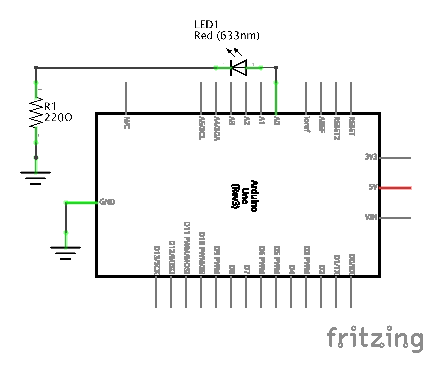
\includegraphics[width=0.7\textwidth]{images/1-LED-A0_sch.pdf}
				\caption{Diagrama esquemático del circuito a ensamblar.}
				\label{dia:anal-uno-sch}
			\end{center}
		\end{figure}

		\begin{marginfigure}
			\begin{center}
				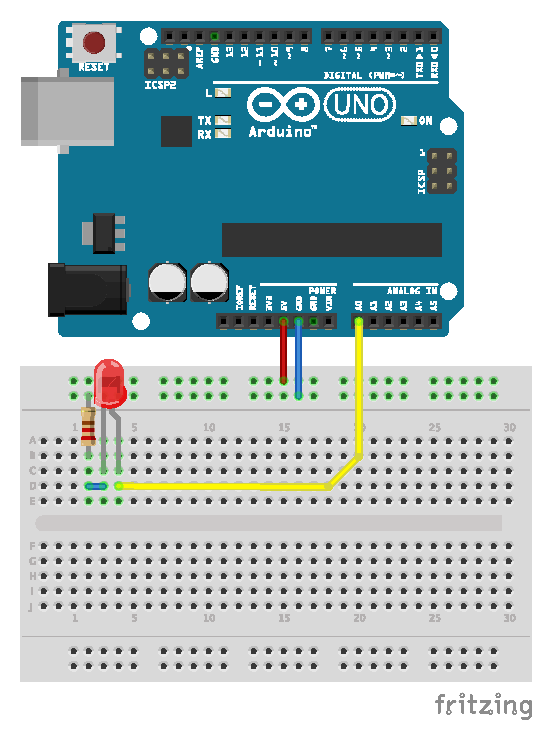
\includegraphics[width=\textwidth]{images/1-LED-A0_bb.pdf}
				\caption{Diagrama representativo del circuito a ensamblar.}
				\label{dia:anal-uno}
			\end{center}
		\end{marginfigure}

    Lo primero que tenemos que hacer es realizar el circuito eléctrico en el protoboard. El circuito lo podemos ver en la figura \ref{dia:anal-uno}; este equema es una representación pictográfica bastante realista del circuito a realizar, sin embargo, en ocasiones puede resultar demasiada información redundante, sobre todo cuando ya se tiene experiencia realizando circuitos eléctricos, por lo que tambien podemos verlo como en la figura \ref{dia:anal-uno-sch} y obtener la misma información.

		\begin{figure}[h]
    	\begin{center}
    		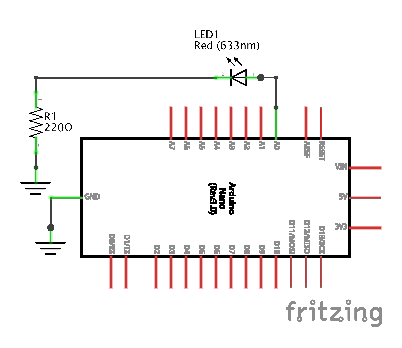
\includegraphics[width=0.7\textwidth]{images/1-LED-A0-nano_sch.pdf}
    		\caption{Diagrama esquemático alternativo del circuito a ensamblar.}
    		\label{dia:anal-nano-sch}
    	\end{center}
    \end{figure}

		\begin{marginfigure}
    	\begin{center}
    		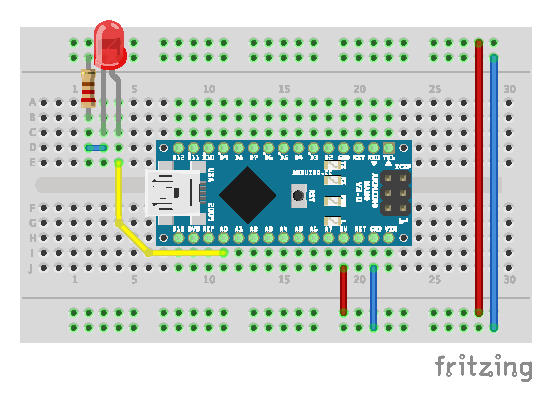
\includegraphics[width=\textwidth]{images/1-LED-A0-nano_bb.pdf}
    		\caption{Diagrama representativo alternativo del circuito a ensamblar.}
    		\label{dia:anal-nano}
    	\end{center}
    \end{marginfigure}

		Si bien la manera mas facil y simple de seguir estas prácticas es con un Arduino UNO, tambien se puede utilizar cualquier otra tarjeta de desarrollo que utilice Wiring-Arduino, por lo que ponemos también un ejemplo con la tarjeta de desarrollo Arduino NANO en la figura \ref{dia:anal-nano}, así como su diagrama esquemático correspondiente en la figura \ref{dia:anal-nano-sch}.

		Nota que los diagramas especifican el cable de conexion al arduino en $A0$, sin embargo, de acuerdo a los ejemplos es necesario conectar el LED en diferentes pines del Arduino y en algunos casos multiples LED.

%-------------------------------------------------------------------------------
%	CONCLUSIONES
%-------------------------------------------------------------------------------

\section{Conclusiones}
	El alumno deberá describir sus conclusiones al final de su reporte de práctica.

%-------------------------------------------------------------------------------
%	HOJA DE ANOTACIONES
%-------------------------------------------------------------------------------

\clearpage
\section{Hoja de Anotaciones}

	Anota los pasos a seguir para utilizar correctamente la fuente de alimentación. \\ \vspace{3cm}% \\ \\ \\ \\ \\ \\

	Anota los pasos a seguir para utilizar correctamente el multímetro como Vóltmetro. \\ \vspace{3cm}% \\ \\ \\

	Carga el ejemplo del IDE de Arduino ubicado en Menu principal, Archivo, Ejemplos, 03. Analog, Fading y modifica el diagrama esquemático de la figura \ref{dia:anal-uno-sch} para que el ejemplo funcione. \\ \vspace{5cm}

	Diseña un circuito eléctrico en el cual 3 LEDs esten conectados a 3 pines del Arduino y se enciendan cuando estos pines del Arduino tengan un voltaje de $5V$. \\ \vspace{5cm}

	Diseña un programa de Arduino que prenda secuencialmente los 3 LEDs dejandolos encendidos $1s$, $1s$, y $2s$

	\begin{multicols}{2}
		Integrantes del equipo: \\[0.4cm]
		\horrule{0.5pt} \\[0.4cm] % Linea horizontal delgada
		\horrule{0.5pt} % Linea horizontal delgada

		Revisó: \\[1.25cm]
		\horrule{0.5pt} \\% Linea horizontal delgada
	\end{multicols}




%-------------------------------------------------------------------------------
%	FIN DEL DOCUMENTO
%-------------------------------------------------------------------------------

\end{document}
